%%%%%%%%%%%%%%%%%%%%%%%%%%%%%%%%%%%%%%%%%
% Short Sectioned Assignment
% LaTeX Template
% Version 1.0 (5/5/12)
%
% This template has been downloaded from:
% http://www.LaTeXTemplates.com
%
% Original author:
% Frits Wenneker (http://www.howtotex.com)
%
% License:
% CC BY-NC-SA 3.0 (http://creativecommons.org/licenses/by-nc-sa/3.0/)
%
%%%%%%%%%%%%%%%%%%%%%%%%%%%%%%%%%%%%%%%%%

%----------------------------------------------------------------------------------------
%	PACKAGES AND OTHER DOCUMENT CONFIGURATIONS
%----------------------------------------------------------------------------------------

\documentclass[paper=a4, fontsize=11pt]{scrartcl} % A4 paper and 11pt font size

\usepackage[T1]{fontenc} % Use 8-bit encoding that has 256 glyphs
%\usepackage{fourier} % Use the Adobe Utopia font for the document - comment this line to return to the LaTeX default
\usepackage[english]{babel} % English language/hyphenation
\usepackage{amsmath,amsfonts,amsthm} % Math packages
\usepackage{graphicx}
\usepackage{lipsum} % Used for inserting dummy 'Lorem ipsum' text into the template
\usepackage{comment}

\usepackage{sectsty} % Allows customizing section commands
\allsectionsfont{\centering \normalfont\scshape} % Make all sections centered, the default font and small caps

\usepackage{fancyhdr} % Custom headers and footers
\pagestyle{fancyplain} % Makes all pages in the document conform to the custom headers and footers
\fancyhead{} % No page header - if you want one, create it in the same way as the footers below
%\fancyfoot[L]{} % Empty left footer
%\fancyfoot[C]{} % Empty center footer
%\fancyfoot[R]{\thepage} % Page numbering for right footer
\renewcommand{\headrulewidth}{0pt} % Remove header underlines
\renewcommand{\footrulewidth}{0pt} % Remove footer underlines
\setlength{\headheight}{13.6pt} % Customize the height of the header

\numberwithin{equation}{section} % Number equations within sections (i.e. 1.1, 1.2, 2.1, 2.2 instead of 1, 2, 3, 4)
\numberwithin{figure}{section} % Number figures within sections (i.e. 1.1, 1.2, 2.1, 2.2 instead of 1, 2, 3, 4)
\numberwithin{table}{section} % Number tables within sections (i.e. 1.1, 1.2, 2.1, 2.2 instead of 1, 2, 3, 4)

\setlength\parindent{0pt} % Removes all indentation from paragraphs - comment this line for an assignment with lots of text

%----------------------------------------------------------------------------------------
%	TITLE SECTION
%----------------------------------------------------------------------------------------

%\newcommand{\horrule}[1]{\rule{\linewidth}{#1}} % Create horizontal rule command with 1 argument of height

%\title{	
%\normalfont \normalsize 
%\textsc{university, school or department name} \\ [25pt] % %Your university, school and/or department name(s)
%\horrule{0.5pt} \\[0.4cm] % Thin top horizontal rule
%\huge Assignment Title \\ % The assignment title
%\horrule{2pt} \\[0.5cm] % Thick bottom horizontal rule
%}

%\author{John Smith} % Your name

%\date{\normalsize\today} % Today's date or a custom date

\begin{document}

%\maketitle % Print the title

%----------------------------------------------------------------------------------------
%	PROBLEM 1
%----------------------------------------------------------------------------------------

\section*{EF-ROM report}
\section*{Xuping Xie}

\section{EF-ROM-DF}
The following are burgers equation,
\begin{eqnarray}
  \left\{\begin{array}{ll}
  u_t-\nu u_{xx}+\overline{u}u_x=f& x\in\Omega,\\
  u(x,0)=u_0(x)& x\in\Omega,\\
  u(x,t)=g(x,t)&  x\in\partial\Omega
  \end{array} \right.
 \end{eqnarray}
where $\nu$ is the diffusion parameter, $f$ the forcing term, $\Omega\subset R$ the computational domain, $t\in[0,T]$. 
\begin{eqnarray}
u_0(x)=\left\{\begin{array}{ll}
1&  x\in(0,\frac{1}{2}],\\
0&  x\in(\frac{1}{2},1).
\end{array}
\right.
\end{eqnarray}
where $\nu=10^{-3}$, domain $x\in[0,1]$, time interval $t\in[0,1]$.  The boundary conditions are homogeneous Dirichlet $u(0,t)=u(1,t)=0$ for all $t$, the forcing term $f=0$. The following parameters were used in the computation $\Delta x=1/1024$;  time-step $\Delta t=10^{-3}$ with Backward Euler in DNS, $\Delta t=10^{-4}$ with Forward Euler in EF-ROM and L-ROM; number of snapshots m=101 (i.e. saved at every 10 step in DNS).
\begin{figure}[htp]
\centering
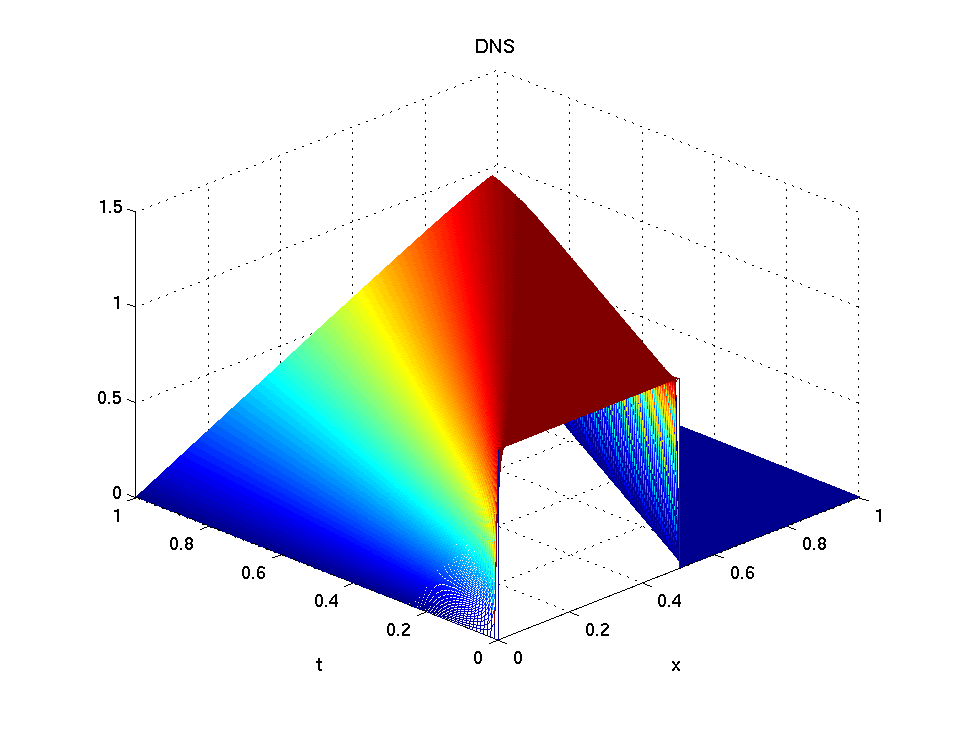
\includegraphics[width=4in]{DNS.eps}
\caption{this is the DNS solution}
\end{figure}
%\begin{figure}[htp]
%\includegraphics[width=2.8in]{EF-ROMDave.eps}
%\includegraphics[width=2.8in]{EF-ROMXuping.eps}
%\caption{The left is Dave's format, the right is the L2-error}
%\end{figure} 
the above figure indicates optimal $\delta=0.0003$, and $\delta=0.0006$. Then, we check the time evolution:
%\begin{figure}
%\includegraphics[width=2.8in]{EF-EvoluDave.eps}
%\includegraphics[width=2.8in]{EF-EvoluXuping.eps}
%\caption{the time evolution of L2-norm(Kinetic Energy)}
%\end{figure} 
From the above the optimal $\delta=0.0003$.
\clearpage
\section{POD-Leray-DF}
I used $r=6,10,20$. The optimal for each one is pretty close. See the following picture 2.1.

So, according to optimal $L^2$ error, the optimal around $\delta=0.135$. I plot the time-evolution, for $\delta=0.135$ and $\delta=0.5$.see fig.2.2
 
\clearpage
From the above, we know that, $\Delta t= 1/10000$, as $\delta$ increase, the solution becomes bad.  BUT, when we try $\Delta t= 1/30000$. 
\section{EF-ROM-Projection}
For EF-ROM-projection, I did 2 test, one is for $r=6$ while $R=2,4,5$, another is for $r=20$, $R=5,10,15$. I also calculated the kinetic energy at each time level. My results show that IF r and R are small, the results are bad. BUT if r and R are large, EF-ROM-projection can still be good. 
see the plots 3.1, 3.2.

\section{POD-Leray-Projection}
For Leray-Projection, those results are good if we choose R is pretty close to r.  It doesn't matter how large r it is. see plots 4.1, 4.2.
%------------------------------------------------

%----------------------------------------------------------------------------------------

\end{document}
